\subsubsection*{\underline{\textsc{\Large Snow Owlbear}}}
\noindent\emph{Large beast, neutral}

It's an owlbear formed entirely of snow.

\noindent\rule{0.5\textwidth}{0.5pt}

\noindent\textbf{Armor Class}: 15

\noindent\textbf{Hit Points}: 88

\noindent\textbf{Speed}: 60 ft.

\noindent\rule{0.5\textwidth}{0.5pt} \\
\begin{table}[H]
	\begin{tabular}{cccccc}
		\textbf{STR} & \textbf{DEX} & \textbf{CON} & \textbf{INT} & \textbf{WIS} & \textbf{CHA} \\
		18 (+4) & 10 (+0) & 16 (+3) & 7 (-2) & 10 (+0) & 3 (-4) \\
	\end{tabular}
\end{table}
\noindent\rule{0.5\textwidth}{0.5pt} \\

\noindent\textbf{Damage Vulnerabilities}: fire

\noindent\textbf{Damage Immunities}: cold

\noindent\textbf{Condition Immunities}: charmed, frightened, paralyzed, poisoned

\noindent\textbf{Senses}: darkvision 60 ft., passive Perception 11

\noindent\textbf{Languages}: Does not speak

\noindent\textbf{Challenge}: 4 (1,100 XP)

\noindent\rule{0.5\textwidth}{0.5pt}

\noindent\textbf{ACTIONS}

\noindent\textbf{Ice Claws}: Melee Ranged Attack: +5 to hit, reach 20 ft., one target. Hit: 17 (4d6 + 3) cold damage. Targets must succeed a DC 12 constitution saving throw or be slowed by the cold (half movement speed).

\noindent\textbf{Snow Prison}: Bonus Action: Target is trapped in a prison of snow from the waist down immobilized (can still perform actions but no movement). Target must succeed a DC 12 dexterity saving throw or take 2d6 + 3 (half on successful save) bludgeoning damage and be immobilized. If immobilized, target must use their movement and succeed a DC 12 strength saving throw to break free.

\noindent\textbf{Blizzard}: Bonus Action, Concentration: Creates a blizzard in a diameter of 30 ft around a location. Visibility inside the blizzard is very low, and targets getting caught in the blizzard get knocked down (take 1d6 of damage).

\noindent\textbf{Snow Pounce}: Bonus Action: The Snow owlbear pounces in the direction of its target, and dives into the snow. The owlbear resurfaces on his next turn but leaves behind two evil snowmen. While the owlbear is under the snow, it is not visible unless revealed with some magic spell. When it resurfaces, all targets in a 10ft radius around the owlbear take (3d8 + 4) cold damage. Any target directly under the owlbear gets knocked to the side and takes an additional 1d6 bludgeoning damage. This ability can be dodged if the target moves out of the way before it resurfaces.

\begin{center}
	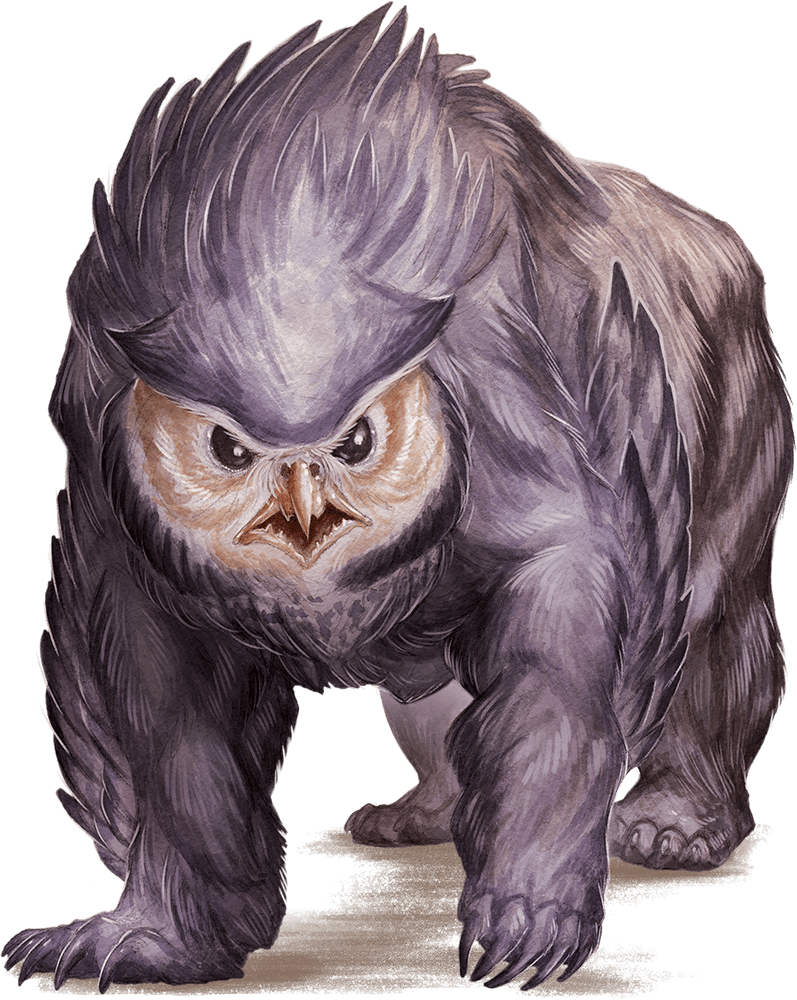
\includegraphics[width = 0.3\textwidth]{owlbear}
	
	\emph{Snow Owlbear}
\end{center}